\documentclass[conference]{IEEEtran}
\IEEEoverridecommandlockouts
% The preceding line is only needed to identify funding in the first footnote. If that is unneeded, please comment it out.
\usepackage{cite}
\usepackage{amsmath,amssymb,amsfonts}
\usepackage{algorithmic}
\usepackage[spanish]{babel}
\usepackage[utf8]{inputenc}
\usepackage{graphicx}
\usepackage{textcomp}
\usepackage{xcolor}
\def\BibTeX{{\rm B\kern-.05em{\sc i\kern-.025em b}\kern-.08em
    T\kern-.1667em\lower.7ex\hbox{E}\kern-.125emX}}
\begin{document}

\title{
{\large \textsc{Escuela Superior Politécnica del Litoral}\\
Conmutación y Enrutamiento - TLMG1009: Proyecto Final
}\\
Sistemas de Respaldos Diarios Automáticos\\
}

\author{\IEEEauthorblockN{\textbf{Lino Ontano}}
\IEEEauthorblockA{	\textit{Telemática}
\\Guayaquil - Ecuador \\
lontano@espol.edu.ec
}
\and
\IEEEauthorblockN{\textbf{Julio Bodero}}
\IEEEauthorblockA{	\textit{Telemática}
\\Guayaquil - Ecuador \\
jcbodero@espol.edu.ec
}
\and
\IEEEauthorblockN{\textbf{Cesar Navas}}
\IEEEauthorblockA{	\textit{Telemática}
\\Guayaquil - Ecuador \\
cesanava@espol.edu.ec
}
\and
\IEEEauthorblockN{\textbf{Josue Martínez}}
\IEEEauthorblockA{	\textit{Telemática}
\\Guayaquil - Ecuador \\
josvmart@espol.edu.ec
}
\and
\IEEEauthorblockN{\textbf{Eduardo Veintimilla}}
\IEEEauthorblockA{	\textit{Telemática}
\\Guayaquil - Ecuador \\
edujvein@espol.edu.ec
}
}


\maketitle

\begin{abstract}
	Este proyecto permitirá explicar el funcionamiento del proyecto realizado, las herramientas utilizadas y las configuraciones pertinentes en los dispositivos intermediarios para poder realizar el respaldo y la consulta.
\end{abstract}

\section{Introducción}\label{sec:int}
Es necesario en una empresa, sea de grande o pequeña escala, tener las redes de sus sucursales siempre disponibles; de esta manera se garantiza el servicio que ofrece y el soporte a su empresa sin importar en que sucursal se encuentre el problema. Existen varias soluciones para mantener la alta disponibilidad de nuestra empresa, pero el riesgo de fallo siempre existirá y es ahí cuando el ingeniero de networking debe tener la solución disponible en un tiempo corto de respuesta. Por eso, la configuración de los dispositivos intermediarios de nuestra red es importante que esté al alcance de la persona encargada de dar soporte a la empresa, sin importar donde se encuentre. Este proyecto permite acceder a la configuración de los equipos intermediarios de nuestra red, en este caso utilizamos de ejemplo una red con tres dispositivos intermediarios, dos sucursales y una matriz. El aplicativo elaborado en el presente proyecto permite realizar un sistema de respaldo diario de estos dispositivos, así como una consulta de los mismos por fecha o por dispositivo. De esta manera ofrecemos una base de datos que servirá para ayudar a mitigar los problemas de fallas ya que se podrá acceder a los archivos de configuración de cualquier sucursal e identificar una posible mala configuración o un mal funcionamiento del mismo.
\begin{figure}[h]
	\centerline{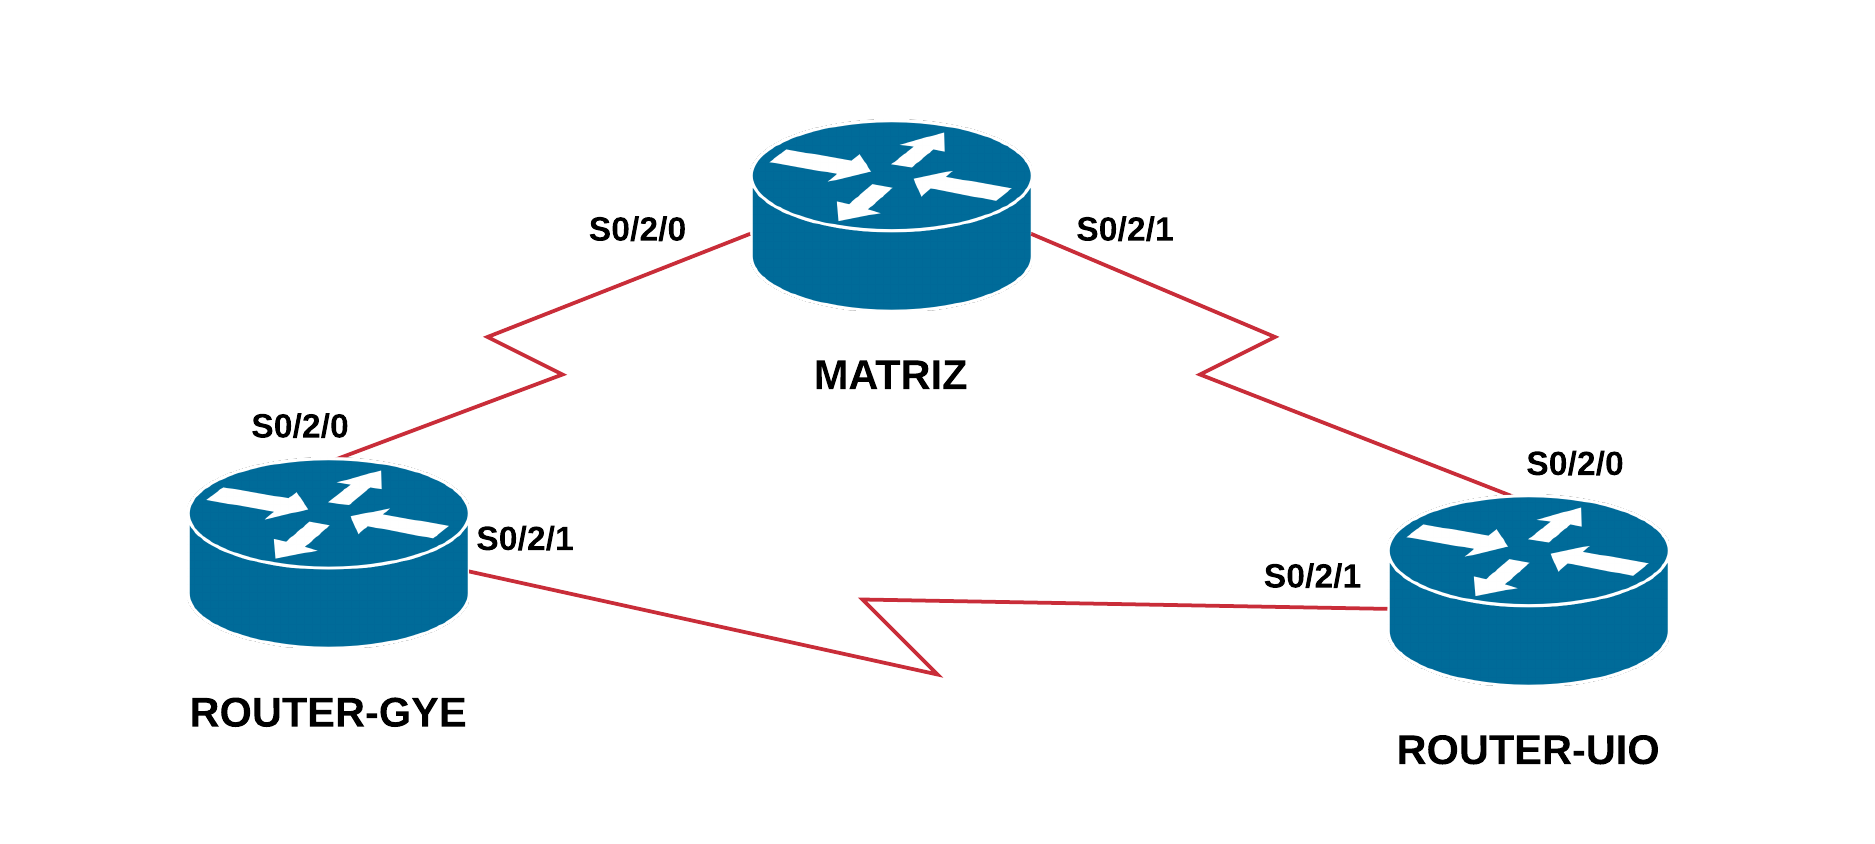
\includegraphics[width=0.51\textwidth]{img/int01.png}}
	\caption{Diagrama de red de las sucursales a respaldar}
	\label{fig:ant00}
\end{figure}
\section{Antecedentes}\label{sec:ant}
\subsection{\textbf{ Dispositivos intermediarios:}}
Los dispositivos intermediarios interconectan dispositivos finales. Estos dispositivos proporcionan conectividad y operan detrás de escena para asegurar que los datos fluyan a través de la red. Los dispositivos intermediarios conectan los hosts individuales a la red y pueden conectar varias redes individuales para formar una internetwork.\\
Los siguientes son ejemplos de dispositivos de red intermediarios:
\begin{itemize}
\item Acceso a la red (switches y puntos de acceso inalámbrico)
\item Internetworking (routers)
\item Seguridad (firewalls)
\end{itemize}

\subsection{\textbf{Protocolo SSH:}}
\begin{figure}[h]
	\centerline{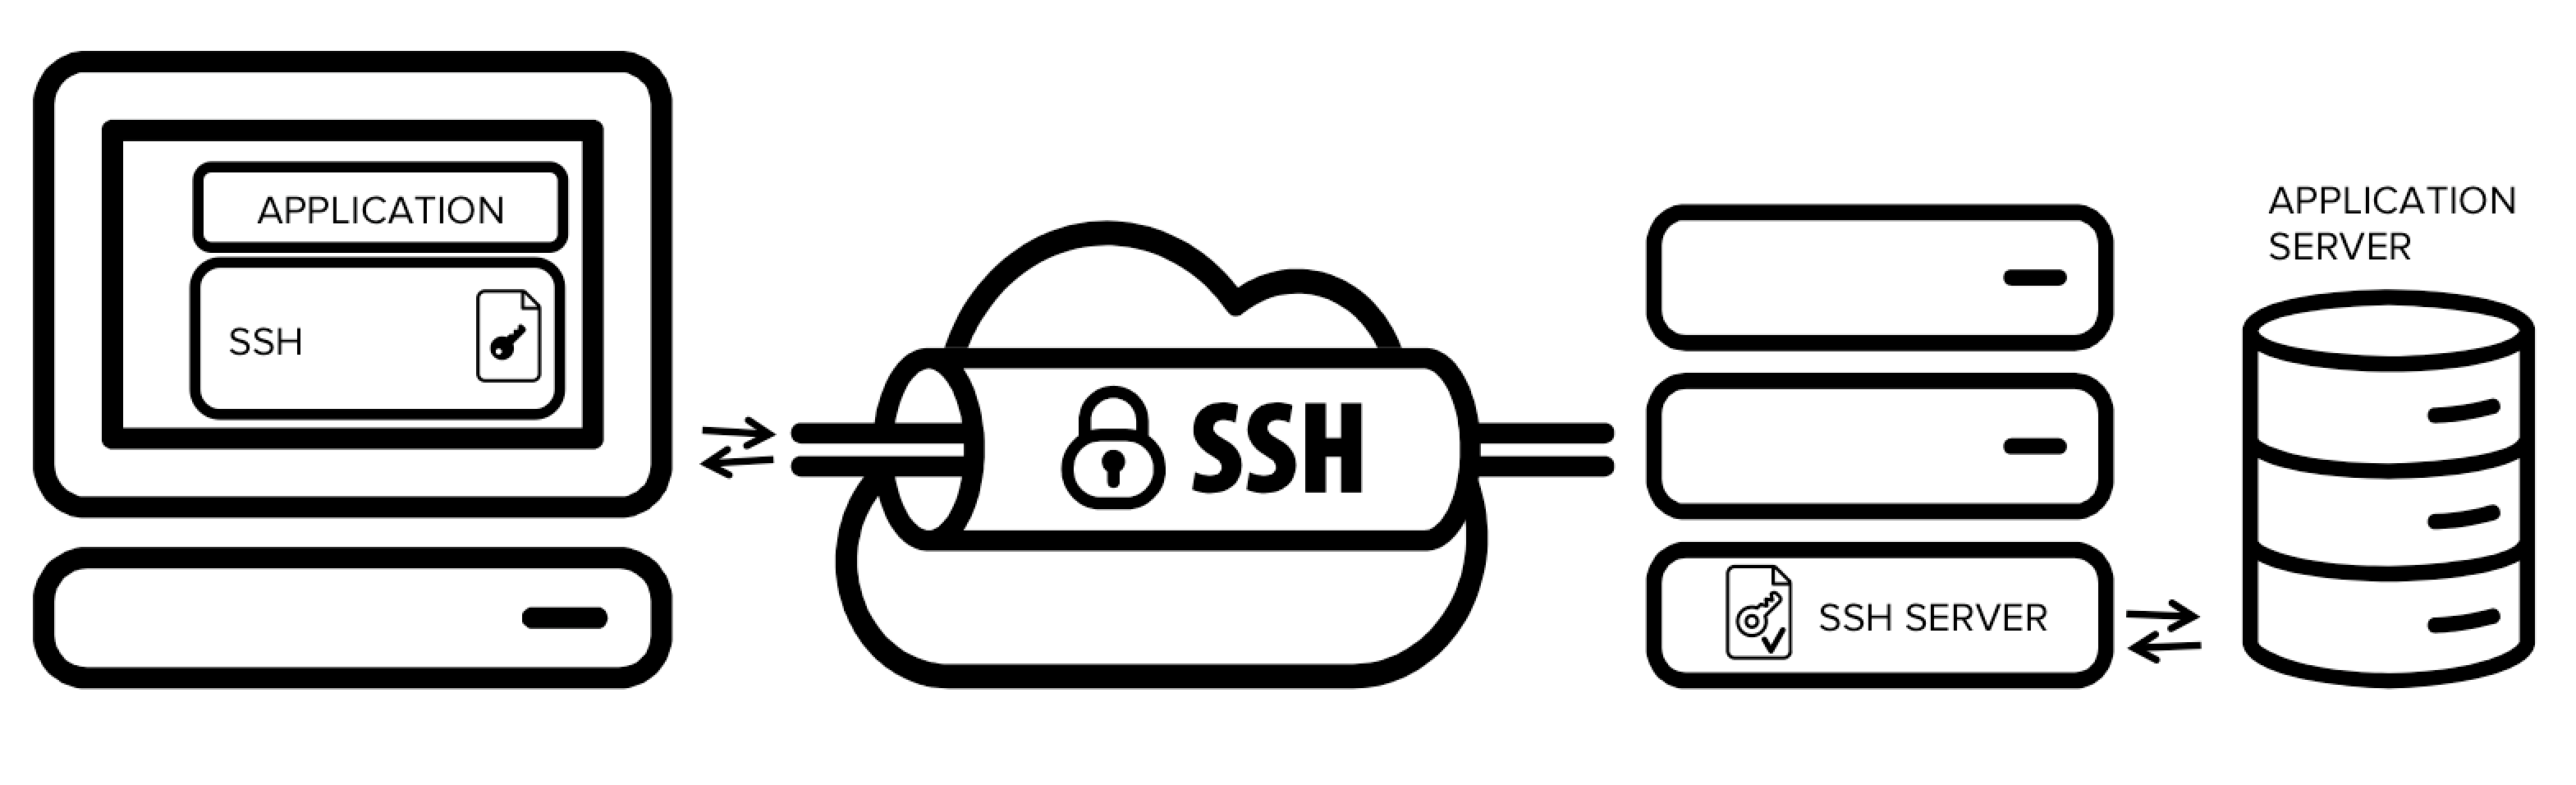
\includegraphics[width=0.45\textwidth]{img/ant02.png}}
	\caption{Funcionamiento del protocolo SSH}
	\label{fig:ant02}
\end{figure}

SSH (o \textit{Secure SHell}) es el nombre de un protocolo y del programa que lo implementa cuya principal función es el acceso remoto a un servidor por medio de un canal seguro en el que toda la información está cifrada. SSH trabaja de forma similar a como se hace con \textit{telnet}. La diferencia principal es que SSH usa técnicas de cifrado que hacen que la información que viaja por el medio de comunicación vaya de manera no legible, evitando que terceras personas puedan descubrir el usuario y contraseña de la conexión ni lo que se escribe durante toda la sesión; aunque es posible atacar este tipo de sistemas por medio de ataques de REPLAY y manipular así la información entre destinos. El protocolo TCP asignado es el 22.

\subsection{\textbf{ Protocolo de Transferencia de Archivos FTP:}}
FTP es un protocolo de red para la transferencia de archivos entre sistemas conectados a una red TCP (Transmission Control Protocol), basado en la arquitectura cliente-servidor. Desde un equipo cliente se puede conectar a un servidor para descargar archivos desde él o para enviarle archivos, independientemente del sistema operativo utilizado en cada equipo.\\
El servicio FTP es ofrecido por la capa de aplicación del modelo de capas de red TCP/IP al usuario, utilizando normalmente el puerto de red 20 y el 21. Un problema básico de FTP es que está pensado para ofrecer la máxima velocidad en la conexión, pero no la máxima seguridad, ya que todo el intercambio de información, desde el login y password del usuario en el servidor hasta la transferencia de cualquier archivo, se realiza en texto plano sin ningún tipo de cifrado, con lo que un posible atacante puede capturar este tráfico, acceder al servidor y/o apropiarse de los archivos transferidos.

\textit{Asterisk} incluye muchas características que anteriormente sólo estaban disponibles en costosos sistemas propietarios PBX, como buzón de voz, conferencias, IVR, distribución automática de llamadas, y otras muchas. Los usuarios pueden crear nuevas funcionalidades escribiendo un dialplan en el lenguaje de script de \textit{Asterisk} o añadiendo módulos escritos en lenguaje C o en cualquier otro lenguaje de programación soportado en GNU/Linux.\\
Uno de los puntos fuertes del software \textit{Asterisk} es que permite la unificación de tecnologías: VoIP, GSM y PSTN.\\
\textit{Asterisk} se empieza a adoptar en algunos entornos corporativos como una gran solución de bajo coste junto con SER (Sip Express Router).


\subsection{\textbf{ OSPF:}}
\textit{Open Shortest Path First} (OSPF), Primer Camino Más Corto, es un protocolo de red para encaminamiento jerárquico de pasarela interior o Interior Gateway Protocol (IGP), que usa el algoritmo Dijkstra, para calcular la ruta más corta entre dos nodos.\\
Su medida de métrica se denomina cost, y tiene en cuenta diversos parámetros tales como el ancho de banda y la congestión de los enlaces. OSPF construye además una base de datos enlace-estado (Link-State Database, LSDB) idéntica en todos los routers de la zona.\\
Una red OSPF se puede descomponer en regiones (áreas) más pequeñas. Hay un área especial llamada área backbone que forma la parte central de la red a la que se encuentran conectadas el resto de áreas de la misma. Las rutas entre las diferentes áreas circulan siempre por el backbone, por lo tanto todas las áreas deben conectar con el backbone. Si no es posible hacer una conexión directa con el backbone, se puede hacer un enlace virtual entre redes.

\section{Desarrollo del concepto}\label{sec:ddc}
\begin{figure}[h]
	\centerline{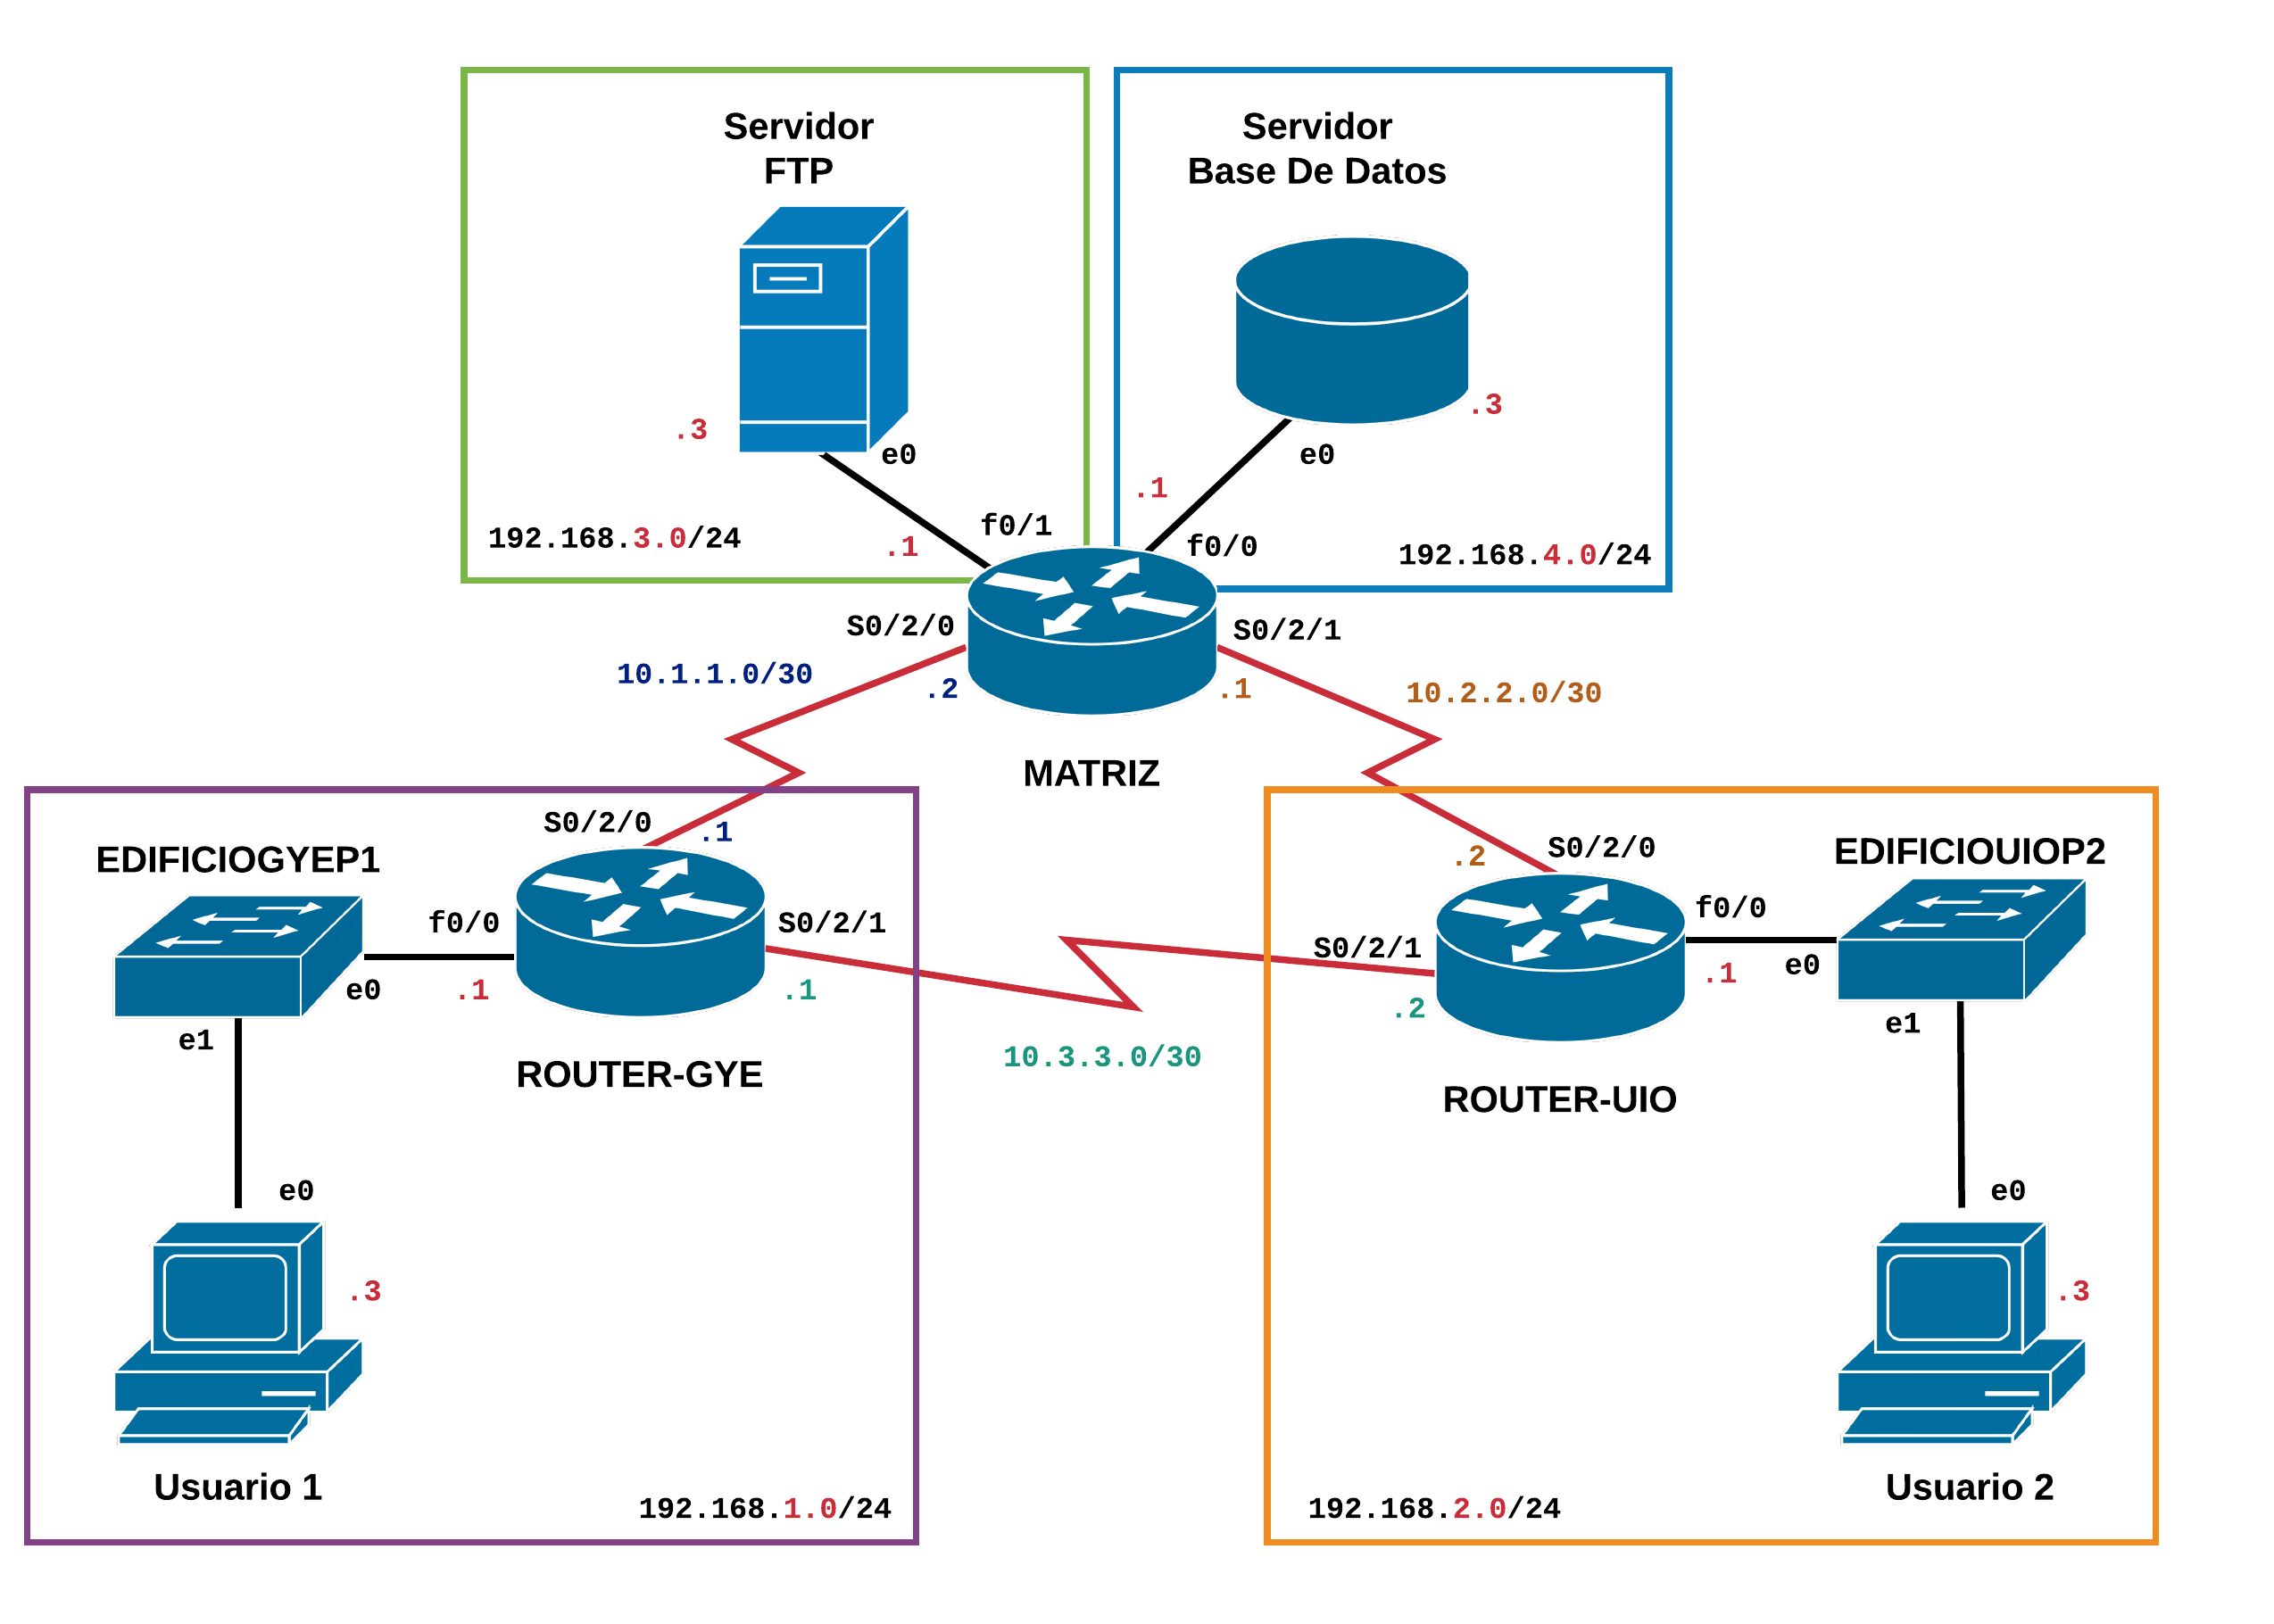
\includegraphics[width=0.50\textwidth]{img/desa01.png}}
	\caption{Diagrama completo de red de nuestra empresa. Se observa que los dispositivos intermediarios interconectan dos sucursales diferentes con la matriz.}
	\label{fig:ddc01}
\end{figure}

Para el desarrollo de nuestro proyecto, nos basamos en la red de la figura \ref{fig:ddc01}, donde planteamos que desde cualquier red de las sucursales, por medio de un aplicativo, poder consultar a cualquier dispositivo intermediario presente de la red y hacer respaldos y consultas de los mismos. Para ello, el aplicativo cuenta con autenticación para ser utilizado, es decir la empresa tendrá una base de datos de usuarios que pueden realizar la gestión de resplado y consultas por medio del aplicativo, además de descargar dichos archivos de consultas. Todo estas conexiones se realizan por medio del protocolo SSH, que nos permite hacer conexión y adquirir los datos de los dispositivos intermediarios de manera segura.

\section{Diseño e Implementación}

\begin{table}[tbp]
\begin{center}
	\begin{tabular}{|p{2.5cm}|p{5.5cm}|}
	\hline
	\textbf{Especificaciones} &\textbf{Raspberry Pi3 Modelo B} \\ \hline
	CPU  &1.2GHz 64-bit quad-core ARMv8 \\\hline
	Memoria (SDRAM) &1 GB compartidos con la GPU \\\hline
	Puertos USB &4 \\\hline
	Almacenamiento integrado &MicroSD \\\hline
	Conectividad de red &10/100 Ethernet RJ-45 vía hub USB, Wifi 802.11n, Bluetooth 4.1 \\\hline
	Fuente de alimentación &5 V vía micro USB o GPIO header \\\hline
	Sistemas Operativos Soportados &GNU/Linux: Debian (Raspbian), Fedora (Pidora), Arch Linux (Arch Linux ARM), Slackware Linux, SUSE Linux Enterprise Server for ARM. RISC OS.\\\hline
\end{tabular}\vspace{0.25cm}
\caption{Características Raspeberry Pi 3 Modelo B}
\label{tab:rb01}
\end{center}
\end{table}

	\subsection{Arduino Uno R3}
	El Arduino Uno R3 utiliza el microcontrolador ATmega328. En adición a todas las características de las tarjetas anteriores, el Arduino Uno utiliza el ATmega16U2 para el manejo de USB en lugar del 8U2 (o del FTDI encontrado en generaciones previas). Esto permite ratios de transferencia más rápidos y más memoria. No se necesitan drivers para Linux o Mac (el archivo inf para Windows es necesario y está incluido en el IDE de Arduino).\\
	\textbf{Arduino} es una compañía open source y open hardware, así como un proyecto y comunidad internacional que diseña y manufactura placas de desarrollo de hardware para construir dispositivos digitales y dispositivos interactivos que puedan sensar y controlar objetos del mundo real. \\
	El microcontrolador de la placa se programa usando el “Arduino Programming Language” (basado en Wiring) y el “Arduino Development Environment” (basado en Processing). Los proyectos de Arduino pueden ser autonomos o se pueden comunicar con software en ejecución en un ordenador (por ejemplo con Flash, Processing, MaxMSP, etc.).
	\begin{figure}[h]
	%\centerline{\includegraphics[width=0.25\textwidth]{platform/ardui}}
	\caption{Arduino Uno R3.}
	\label{fig:ardui}
	\end{figure}
	 El precio en Amazon oscila entre los 12 y 30 dólares, dependiendo del kit a comprar.\\
	Las características principales están presentes en el cuadro \ref{tab:ardui01}.
	\begin{table}[h]
\begin{center}
	\begin{tabular}{|p{2.5cm}|p{5.5cm}|}
	\hline
	\textbf{Especificaciones} &\textbf{Arduino Uno R3} \\ \hline
	Microcontrolador  &ATmega328 \\\hline
	Voltaje de entrada &7 - 12 V \\\hline
	Entradas digitales &14 pines digitales de I/0 (6 salidas PWM) \\\hline
	Entradas analógicas & 6 entradas análogas \\\hline
	Memoria Flash &32k\\\hline
	Reloj &16MHz \\\hline
	Sistemas Operativos Soportados &N/A.\\\hline
\end{tabular}\vspace{0.25cm}
\caption{Características Arduino Uno R3}
\label{tab:ardui01}
\end{center}
\end{table}
	\subsection{Beaglebone black}
	Es una computadora barebone de desarrollo, la sucesora de la beaglebone lanzada en octubre de 2011. El precio está en 45 dólares y entre otras diferencias incrementa la RAM a 512 MB, el reloj de procesador a 1GHz, y añade HDMI y 2 GB de memoria flash eMMC. También se entrega con kernel Linux 3.8, permitiendo a la BeagleBone Black tener la ventaja del Gestor de Renderizado Directo (DRM).Demás especificaciones se observa en el cuadro \ref{tab:bb01}
		\begin{table}[h]
\begin{center}
	\begin{tabular}{|p{2.5cm}|p{5.5cm}|}
	\hline
	\textbf{Especificaciones} &\textbf{BeagleBone Black} \\ \hline
	CPU  &Cortex-A8 + 2xPRU (200MHz) \\\hline
	Frecuencia SoC &1000MHz \\\hline
	DSP &DDR3 \\\hline
	Memoria & 512 \\\hline
	Memoria Flash &32k\\\hline
	Reloj &16MHz \\\hline
	Sistemas Operativos Soportados &Rowboat,Angstrom, Fedora, FreeBSD, MINIX 3, NetBSD, OpenBSD, openSUSE, QNX, RISC OS, Ubuntu, Void Linux, Windows Embedded.\\\hline
\end{tabular}\vspace{0.25cm}
\caption{Características BeagleBone Black}
\label{tab:bb01}
\end{center}
\end{table}
\begin{figure}[h]
	%\centerline{\includegraphics[width=0.2\textwidth]{platform/bb.jpg}}
	\caption{BeagleBone Black.}
	\label{fig:ant01}
\end{figure}
\subsection{pcDuino}
	\textbf{pcDuino} es una mini computadora o plataforma de computadora de una sola placa que funciona con PC como el sistema operativo, como Ubuntu y Android ICS. Da salida a la pantalla a HDMI. Además, tiene una interfaz de encabezados de hardware compatible con Arduino (TM). pcDuino puede usarse para enseñar Python, C y más cosas interesantes.\\
	\begin{figure}[h]
	%\centerline{\includegraphics[width=0.2\textwidth]{platform/pcd.png}}
	\caption{pcDuino1.}
	\label{fig:ant01}
\end{figure}
	\textit{pcDuino1} es una plataforma de mini PC rentable y de alto rendimiento que ejecuta PC como SO, como Ubuntu y Android ICS. Envía su pantalla a un televisor o monitor habilitado con HDMI a través de la interfaz HDMI incorporada. Está especialmente dirigido a las crecientes demandas de la comunidad de código abierto. La plataforma podría funcionar como un sistema operativo tipo PC completo con una cadena de herramientas fácil de usar y compatible con el popular ecosistema Arduino, como Arduino Shields (puede que necesite un puente protector) y proyectos de código abierto, etc. Las características principales se las observa en el cuadro \ref{tab:pcd01}.\\
			\begin{table}[h]
\begin{center}
	\begin{tabular}{|p{2.5cm}|p{5.5cm}|}
	\hline
	\textbf{Especificaciones} &\textbf{pcDuino1} \\ \hline
	CPU  &1GHz ARM Cortex A8\\\hline
	DRAM &1 GB \\\hline
	Almacenamiento OnBoard &2GB Flash, microSD card slot hasta 32 GB \\\hline
	Interfaz de Red & 10/100Mbps RJ45 y USB Wifi extensión\\\hline
	Alimentación &5V, 2A\\\hline
	Sistemas Operativos Soportados &Linux3.0 + Ubuntu 12.04Android ICS 4.0\\\hline
\end{tabular}\vspace{0.25cm}
\caption{Características pcDuino1}
\label{tab:pcd01}
\end{center}
\end{table}
\section{Comparación de Plataformas}
Cada uno de estas mini computadoras tienen su correcto desarrollo dependiendo del aplicativo en el que le estén usando, es decir su uso dependerá de la función que lo pongas a realizar. La de menor escalabilidad podríamos mencionar a Arduino, ya que en primer lugar es un microcontrolador, y hay cosas en las que se queda corto, pero es ideal para llevar control de todo tipo de sensores y actadores y por su precio más todavía. Los restantes dependerá del sistema operativo a usarse, y los GPIOS que requeramos usar, si queremos un sistema operativo en tiempo real, la tasa de datos que queramos procesar, todas esas consideraciones hay que tener en cuenta al momento de escoger que plataforma utilizar.
\section{Conclusiones}
\begin{itemize}
	\item Las plataformas de prototipado permite elaborar a bajo costo operaciones de hardware por medio de periféricos de manera más sencilla.
	\item La utilización de las plataformas dependerá de la función que quiera realizar.
\end{itemize}

\begin{thebibliography}{00}
\bibitem{b1}  Liz upton, ``Introducing the New Out Of Box Software (NOOBS)'' , Raspberry Pi, 2013.
\bibitem{b2} Shead, Sam, ``Raspberry Pi delivery delays leave buyers hungry (and angry)", ZDNet, Octubre 2012.
\bibitem{b3} GSyC, ``Simple Network Managment Protocol,''  Universidad Rey Juan Carlos, 2013.
\bibitem{b4} LinkSprite, ``pcDuino1 Overview ,''  admin.
\bibitem{b5} ``OMAP3530 BeagleBoard" High perfomance and numerous expansion options; page 3, Dkc1.digikey.com , Mayo 2009.
\end{thebibliography}

\end{document}
